\documentclass[8pt]{beamer}
\usefonttheme[onlymath]{serif}


\setbeamertemplate{frametitle}{%
    \vskip1ex
    \usebeamerfont{frametitle}%
    \insertframetitle
%   \insertsubsectionhead\par        %  ← 원하는 대로 변경 가능
    \vskip1ex
    \hrule                             % 밑줄(선택)
}

% 테마 선택 (선택 사항)
% \usetheme{Madrid} % 기본 테마, 다른 테마 사용 가능
% \font{serif}
\usepackage{amsfonts}
\usepackage{amssymb}
\usepackage[T1]{fontenc} % To use combination of textbf, textit


% \setcounter{MaxMatrixCols}{20}

% (필요한 패키지들)
% \usepackage{amsthm}
\setbeamertemplate{theorems}[numbered]  % 정리, 정의 등에 번호를 달아줌

% \theoremstyle{plain} % insert bellow all blocks you want in italic
% \newtheorem{theorem}{Theorem}[section] % to number according to section
% 
% \theoremstyle{definition} % insert bellow all blocks you want in normal text
% \newtheorem{definition}{Definition}[section] % to number according to section
% \newtheorem*{idea}{Proof idea} % no numbered block
\usepackage{tcolorbox}

% 필요할 경우 패키지 추가
\usepackage{graphicx} % 이미지 삽입을 위한 패키지
\usepackage{amsmath}   % 수식 사용
\usepackage{hyperref}  % 하이퍼링크 추가
\usepackage{cleveref}
\usepackage{multicol}  % 여러 열 나누기
\usepackage{ulem} % 취소선 및줄 나누기

\usepackage{mathtools}



\newcommand{\mrm}[1]{\mathrm{#1}}
\newcommand{\mbb}[1]{\mathbb{#1}}
\newcommand{\mb}[1]{\mathbf{#1}}
\newcommand{\mc}[1]{\mathcal{#1}}
\newcommand{\tb}[1]{\textbf{#1}}
\newcommand{\ti}[1]{\textit{#1}}
\newcommand{\mypois}[1]{\operatorname{Pois}(#1)}

\newcommand{\mybin}[2]{\operatorname{Bin}\!\left(#1,#2\right)}
\newcommand{\mytoinf}[1]{#1 \rightarrow \infty}
\newcommand{\myexp}[1]{\exp{\left(#1\right)}}
\newcommand{\myunif}[2]{\operatorname{Unif}\!\left(#1, #2\right)}
\newcommand{\mygeom}[1]{\operatorname{Geom}\!\left(#1\right)}
\newcommand{\myexpo}[1]{\operatorname{Expo}\!\left(#1\right)}
\newcommand{\abs}[1]{\left\lvert #1 \right\rvert}
\DeclarePairedDelimiter\floor{\left\lfloor}{\right\rfloor}


% 발표 제목, 저자, 날짜 설정
\title{SAC Debugging and Experiment}
\author{Gwanwoo Choi}
% \date{}

\begin{document}
% 표지 슬라이드
\begin{frame}
    \titlepage
\end{frame}

% % 목차 슬라이드
% \begin{frame}
%     \frametitle{Table of Contents}
%     \tableofcontents
% \end{frame}

% \subsection{Continuous Random Variable}

% \begin{frame}
%     \frametitle{Table of Contents}
%     \tableofcontents[currentsubsection]
% \end{frame}


\begin{frame}{Code implementation}
    \begin{figure}
        \centering
        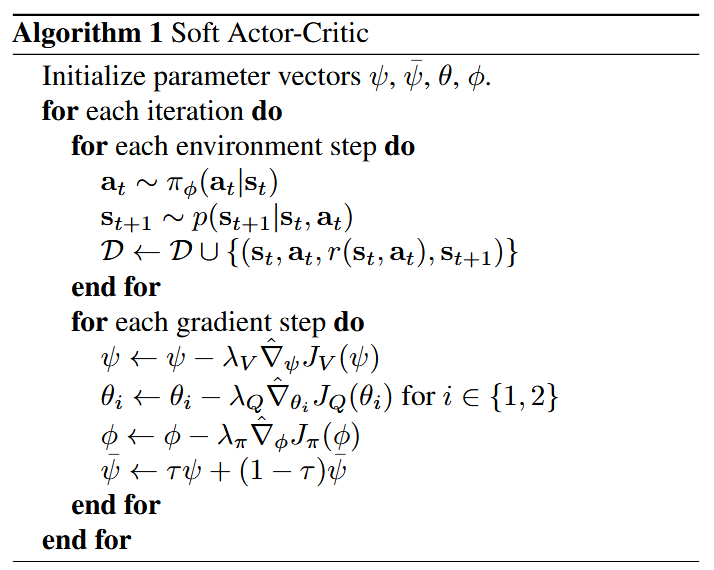
\includegraphics[width=0.7\textwidth]{fig6.png}
    \end{figure}

    I implemented SAC code based on this algorithm.
\end{frame}


% \begin{columns}[c]
%     \begin{column}{0.5\textwidth}
%         \begin{figure}
%             \centering
%             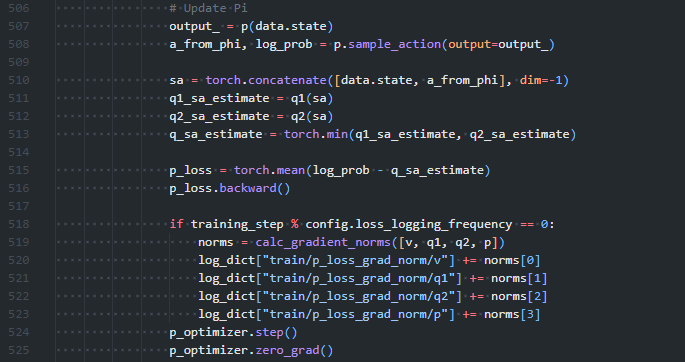
\includegraphics[width=1.0\textwidth]{fig7.png}
%         \end{figure}
%     \end{column}
%     \begin{column}{0.5\textwidth}
%         \begin{figure}
%             \centering
%             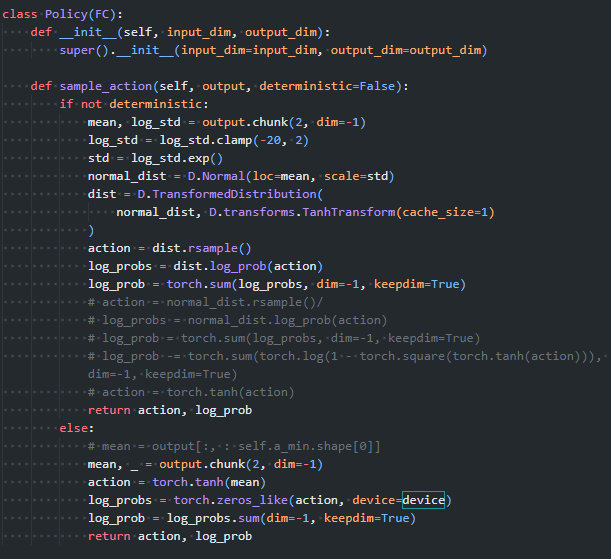
\includegraphics[width=0.9\textwidth]{fig8.png}
%         \end{figure}
%     \end{column}
% \end{columns}





\begin{frame}{Code implementation}
    Network arcitectures are like these
    \begin{columns}[t]
        \begin{column}{0.5\textwidth}            
            \begin{figure}
                \centering
                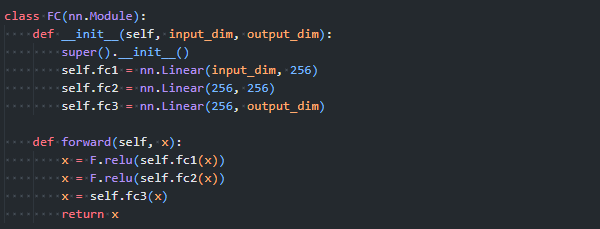
\includegraphics[width=1.0\textwidth]{FCnn.png}
            \end{figure}
            \begin{figure}
                \centering
                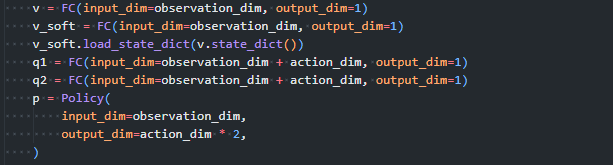
\includegraphics[width=1.0\textwidth]{NetworkArchitectures.png}
            \end{figure}
        \end{column}
        \begin{column}{0.5\textwidth}
            \begin{figure}
                \centering
                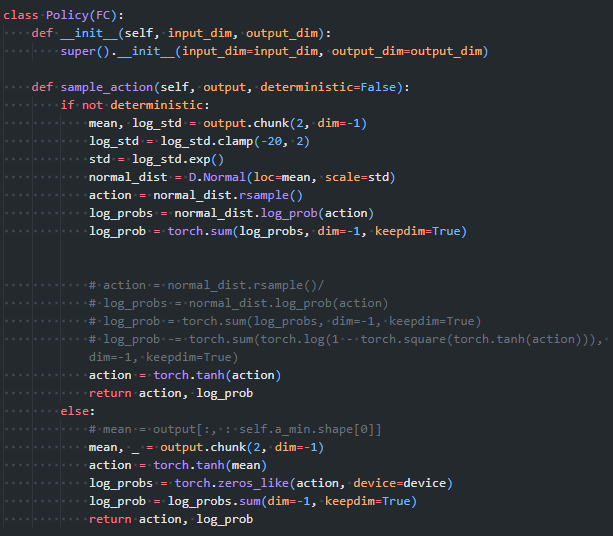
\includegraphics[width=1.0\textwidth]{NotCoVPolicy.png}
            \end{figure}
        \end{column}
    \end{columns}
\end{frame}

\begin{frame}{Code implementation}
    My implementation follows Appendix D of the SAC paper almost exactly
    \begin{figure}
        \centering
        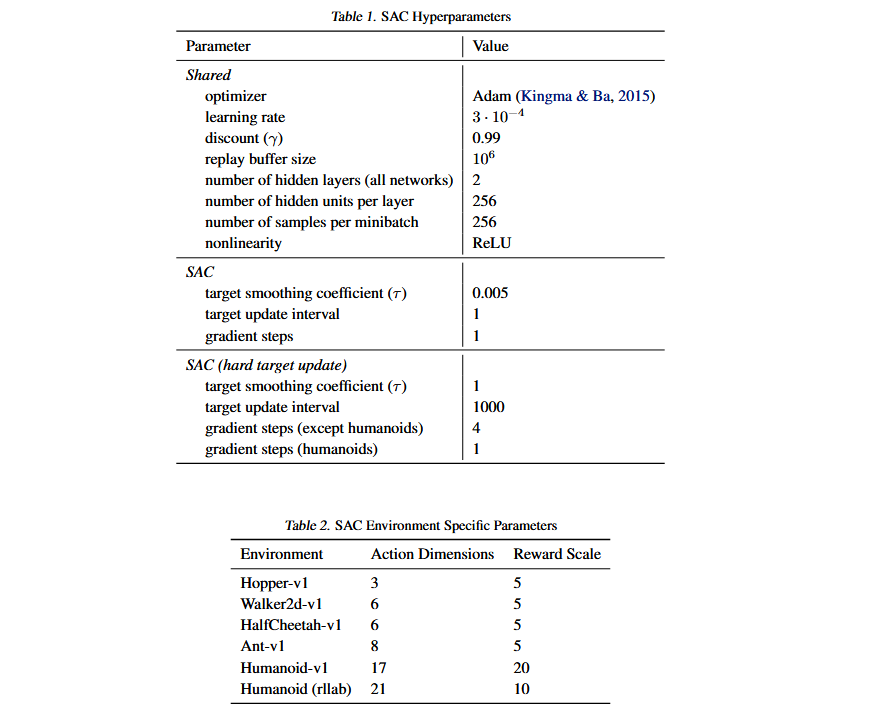
\includegraphics[width=0.8\textwidth]{SACAppendixD.png}
    \end{figure}
\end{frame}

\begin{frame}{Code implementation}
    Update rule for value function $V$ is
    \[
    \begin{gathered}
        J_V(\psi) = \mbb{E}_{s_t \sim \mathcal{D}} \left[ \frac{1}{2}\left(V_\psi (s_t) - \mbb{E}_{a_t \sim \pi_\phi} \left[\min_{\theta} Q_{\theta} (s_t, a_t) - \log{(\pi_\phi (a_t |s_t))}\right]\right)^2\right] \\
        \hat{\nabla}_\psi J_V(\psi) = \nabla_\psi V_\psi (s_t) \left(V_\psi (s_t) - \min_\theta Q_\theta (s_t, a_t) + \log{\pi_\phi (a_t|s_t)}\right)
    \end{gathered}
    \]
    My code implementation is
    \begin{figure}
        \centering
        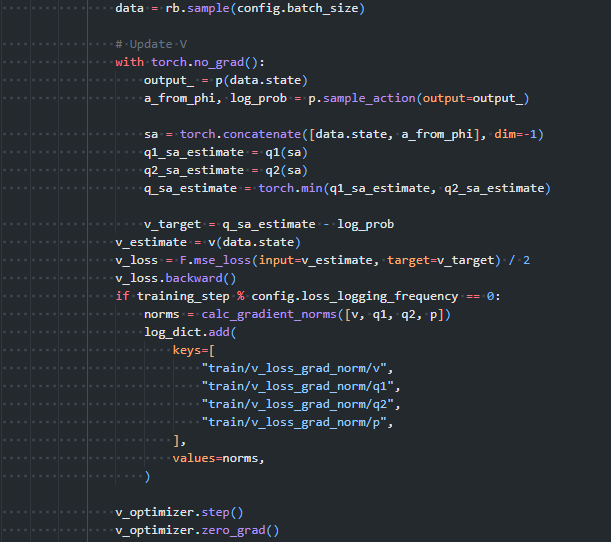
\includegraphics[width=0.55\textwidth]{fig5.png}
    \end{figure}
\end{frame}

\begin{frame}{Code implementation}
    Update rule for action value function $Q_{\theta_i}$ is
    \[
    \begin{gathered}
        J_Q(\theta_i) = \mbb{E}_{(s_t,a_t) \sim \mathcal{D}} \left[ \frac{1}{2} \left( Q_{\theta_i} (s_t, a_t) - r(s_t, a_t) - \gamma \mbb{E}_{s_{t+1}\sim P} [V_{\bar{\psi}} (s_{t+1})] \right)^2\right] \\
        \hat{\nabla}_{\theta_i} J_Q (\theta_i) = \nabla_{\theta_i} Q_{\theta_i} (s_t, a_t) \left(Q_{\theta_i}(s_t, a_t) - r(s_t, a_t) - \gamma V_{\hat{\psi}}(s_{t+1}) \right)
    \end{gathered}
    \]
    My code implementation is
    \begin{figure}
        \centering
        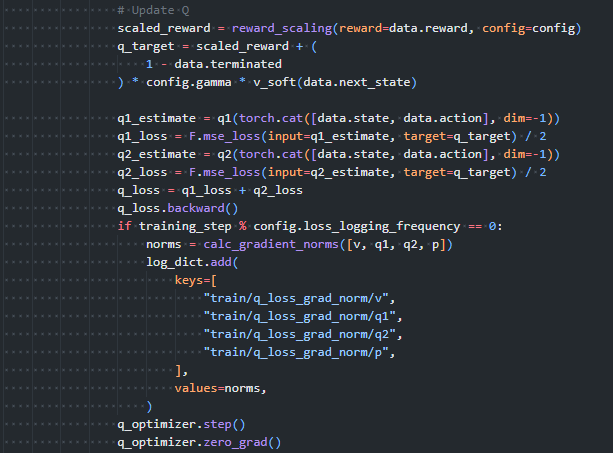
\includegraphics[width=0.63\textwidth]{UpdateQ.png}
    \end{figure}
\end{frame}

\begin{frame}{Code implementation}
    Update rule for policy network $\pi_\phi$ is
    \[
    \begin{gathered}
        J_\pi(\phi) = \mbb{E}_{s_t \sim \mathcal{D}, \epsilon_t \sim \mathcal{N}}[\log{\pi_\phi (f_\phi (\epsilon_t))} - \min_\theta Q_\theta (s_t, f_\phi(\epsilon_t; s_t))] \\
        \begin{aligned}
            \hat{\nabla}_{\phi} J_\pi (\phi) =& \nabla_\phi \log{\pi_\phi (a_t | s_t)}  \\
            &+(\nabla_{a_t} \log{\pi_\phi (a_t |s_t)} - \nabla_{a_t} \min_\theta Q_\theta(s_t, a_t)) \nabla_\phi f_\phi (\epsilon_t; s_t)
        \end{aligned}
    \end{gathered}
    \]

    \begin{columns}
        \begin{column}{0.5\textwidth}
            \begin{figure}
                \centering
                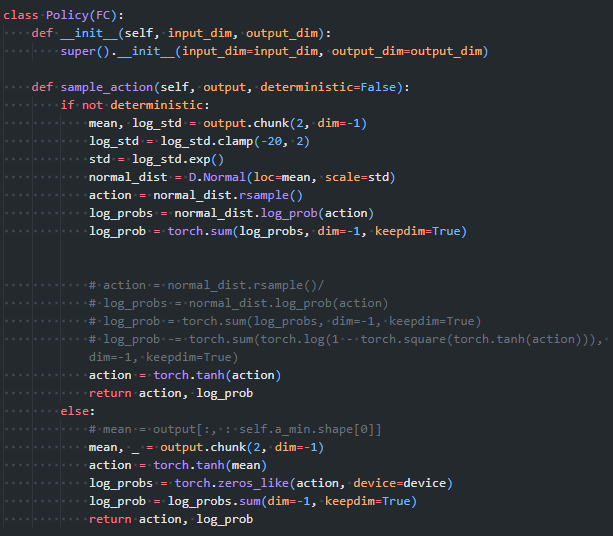
\includegraphics[width=1.0\textwidth]{NotCoVPolicy.png}
            \end{figure}
        \end{column}
        \begin{column}{0.5\textwidth}
            \begin{figure}
                \centering
                \includegraphics[width=1.0\textwidth]{UpdateP.png}
            \end{figure}
        \end{column}
    \end{columns}


    Note that $a_t = f_\phi (\epsilon_t; s_t) = \sigma \epsilon_t + \mu$, where $\mu = \mu_\phi(s_t), \sigma=\sigma_\phi (s_t)$ and $\epsilon_t \sim \mathcal{N}(0, I)$
\end{frame}


\begin{frame}{Reproducibility}
    Reproducibility is very important to compare performance of several experiments
    \begin{figure}
        \centering
        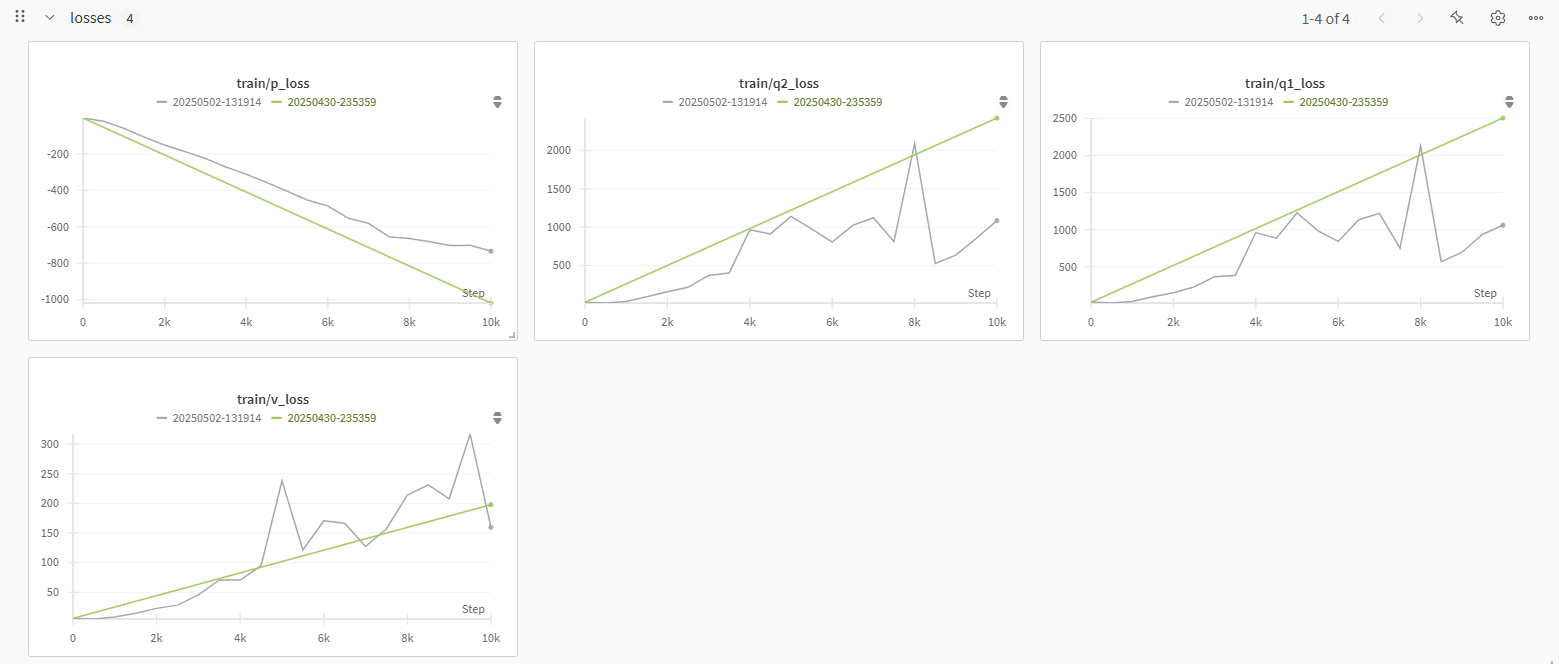
\includegraphics[width=0.8\textwidth]{UnmatchedReprod.png}
    \end{figure}
    I had Non-reproducibility issues between experiments of same settings
    \begin{itemize}
        \item It seems that different training results occur in each workstation(A5000) and desktop (RTX 3060).
    \end{itemize}
    So if one wants to guarantee reproducibility, then it would be nice to run experiments in same devices.
\end{frame}

\begin{frame}{Wrong seed fixing}
    \begin{itemize}
        \item Green one is average of every rewards in one evaluation episode
        \item Pink one is average of every rewrads in ten evaluation episodes
        \item But there exists frequently matched points
    \end{itemize}

    If in each episode start state is different, then
    \begin{itemize}
        \item It seems odd that there exists frequently matched points because usually in each episode, different states, different actions, and different rewards are expected to be represented.
    \end{itemize}

    \begin{figure}
        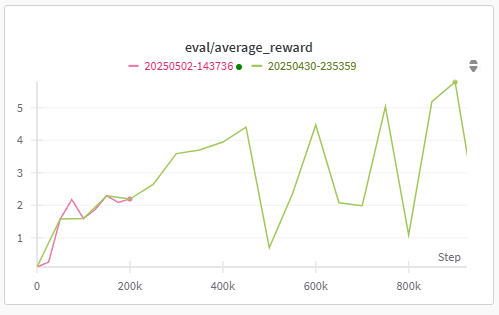
\includegraphics[width=0.7\textwidth]{WrongSeedSetting.png}
    \end{figure}
\end{frame}

\begin{frame}{Wrong seed fixing}
    I had reset with fixed seed in every evaluation episodes
    \begin{figure}
        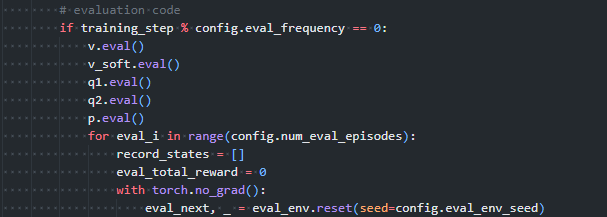
\includegraphics[width=0.8\textwidth]{WrongEvalSeed}
    \end{figure}

    Code should be like these.
    \begin{figure}
        
\includegraphics[width=0.8\textwidth]{FixEvalSeedFix1.png}
    \end{figure}    
    \begin{figure}
        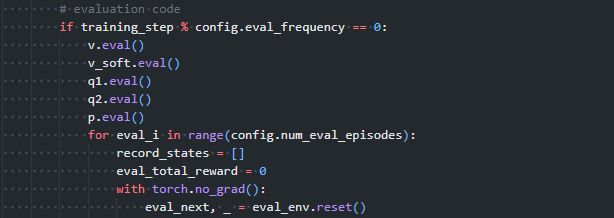
\includegraphics[width=0.8\textwidth]{FixEvalSeedFix2.png}
    \end{figure}
\end{frame}

\begin{frame}{Wrong seed fixing}
    Note:
    \begin{itemize}
        \item From the point env.reset with a specific seed, random sequences are uniquely determined.
        \item For example, suppose we rolled out 100 episodes with starting "env.reset(seed=42)". Then with fixed policy, all state sequences and reward sequences in each episode are same for 100 times.
    \end{itemize}
\end{frame}

\begin{frame}{Change of variables}
    In my first code implementation, 
    \begin{itemize}
        \item Change of variables is not applied
        \item Action range transformation is not applied
    \end{itemize}
    \begin{figure}
        \centering
        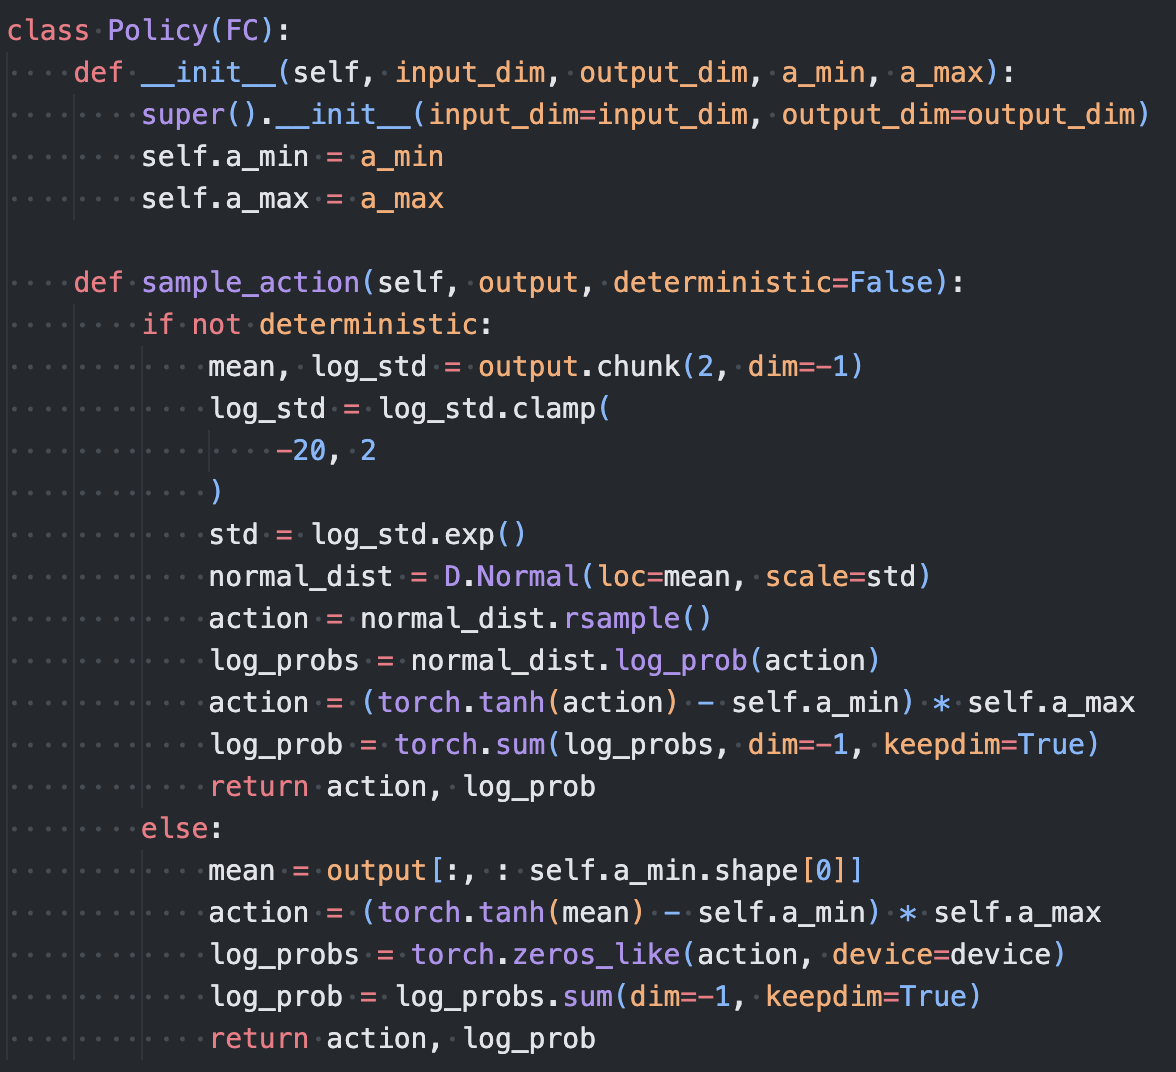
\includegraphics[width=0.7\textwidth]{fig3.png}
    \end{figure}
\end{frame}


\begin{frame}{Change of variables}
    \begin{itemize}
        \item PDF of continuous r.v. $X$ is defined by derivative of CDF
        \item $F(x) = P(X \leq x)$, $f(x) = F^\prime (x)$
    \end{itemize}
    \begin{Theorem}[Change of variables in one dimension]
        Let $X$ be a continuous r.v. with PDF $f_X$, and let $Y=g(X)$, where $g$ is differentiable and strictly increasing or strictly decreasing (invertible). Then the PDF of $Y$ is given by
        \[
        f_Y(y) = f_X(x) \abs{\frac{dx}{dy}}
        \]
        Where $x=g^{-1}(y)$. The support of $Y$ is all $g(x)$ with $x$
    \end{Theorem}

    \bigskip
    \ti{Proof.} If $g$ is strictly increasing, $\frac{dx}{dy} > 0$. $F_Y(y) = P(Y \leq y) = P(g(X) \leq y) = P(X \leq g^{-1}(y)) = F_X(g^{-1}(y)) = F_X(x)$.

    So by chain rule, $f_Y(y) = f_X(x) \frac{d(g^{-1}(y))}{dy} = f_X(x) \frac{dx}{dy} = f_X(x) \abs{\frac{dx}{dy}}$

    If $g$ is strictly decrasing, $\frac{dx}{dy} < 0$.
    $
    F_Y(y) = P(Y \leq y) = P(g(X) \leq y) = P(X \geq g^{-1}(y)) = 1 - F_X(g^{-1}(y)) = 1 - F_X(x)
    $. Then $f_Y(y) = -f_X(x) \frac{dx}{dy} = f_X(x) \abs{\frac{dx}{dy}}$.
\end{frame}

\begin{frame}{Change of variables}
    In SAC, policy $\pi$ is the probability such that $\pi : \mathcal{S} \mapsto \Delta (\mathcal{A})$. But in practice, mujoco environment, which has continuous action space, usually has action range, in which each element of action has range of $(-1, 1)$.

    \bigskip
    For represent continuous distribution with neural network, we usually adopt gaussian distribution $\mu$. Then the r.v. $A^\prime \sim \mu(\cdot | s)$ has relationship with $A \sim \pi(\cdot | s)$ with $A = \tanh{(A^\prime)}$. Since each $\mu$ and $\pi$ is PDF function of $A^\prime$ and $A$, We need to apply change of variables formula.

    \bigskip
    \[
    \begin{gathered}
        \pi(a|s) = \mu(a^\prime | s) \abs{\operatorname{det} \frac{da}{da^\prime}}^{-1}, \frac{da}{da^\prime} = \frac{d\tanh{(a^\prime)}}{da^\prime} = \operatorname{diag}(1 - \operatorname{tanh}^2 (a^\prime)) \\
        \operatorname{log} \pi(a|s) = \operatorname{log} \mu(a^\prime |s) - \sum_{i=1}^D \log{(1 - \operatorname{tanh}^2 (a^\prime_i))}
    \end{gathered}
    \]
\end{frame}

\begin{frame}{Change of variables}
    Fixed version of Policy Network is
    \begin{figure}
        \centering
        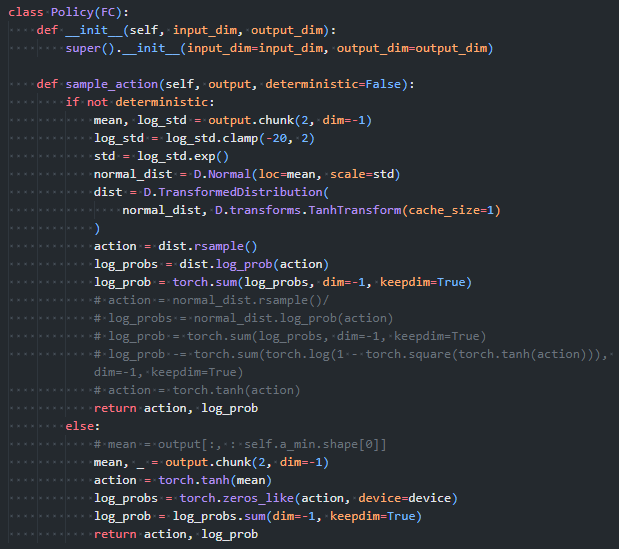
\includegraphics[width=0.7\textwidth]{CoVPolicy.png}
    \end{figure}
\end{frame}

\begin{frame}{Change of variables}
    Performance compare
    \begin{itemize}
        \item Green is the version of adopting change of variable
        \item Cyan is not adopted version
    \end{itemize}
    Fixed version shows slightly better performance than previous version.
    \begin{figure}
        \centering
        \includegraphics[width=0.8\textwidth]{CovReturns.png}
    \end{figure}
\end{frame}

\begin{frame}{Change of variables}
    After adopting change of variables (CoV), q loss value increases

    \begin{itemize}
        \item Adopt CoV version is Pink, and dropped CoV version is Mint
        \item Note that before adopting CoV, the loss function is $\operatorname{log} \mu(a^\prime |s)$, where $\mu$ is gaussian probability density induced by reparametrization trick
        \item and after adopting CoV, the loss function is $\operatorname{log} \mu(a^\prime |s) - \sum_{i=1}^D \log{(1 - \operatorname{tanh}^2 (a^\prime_i))}$
        \item $ \sum_{i=1}^D \log{(1 - \operatorname{tanh}^2 (a^\prime_i))} < 0$ ($\because 0 < \operatorname{tanh}^2 (a^\prime_i) \leq 1$)
    
    \end{itemize}
    \begin{figure}
        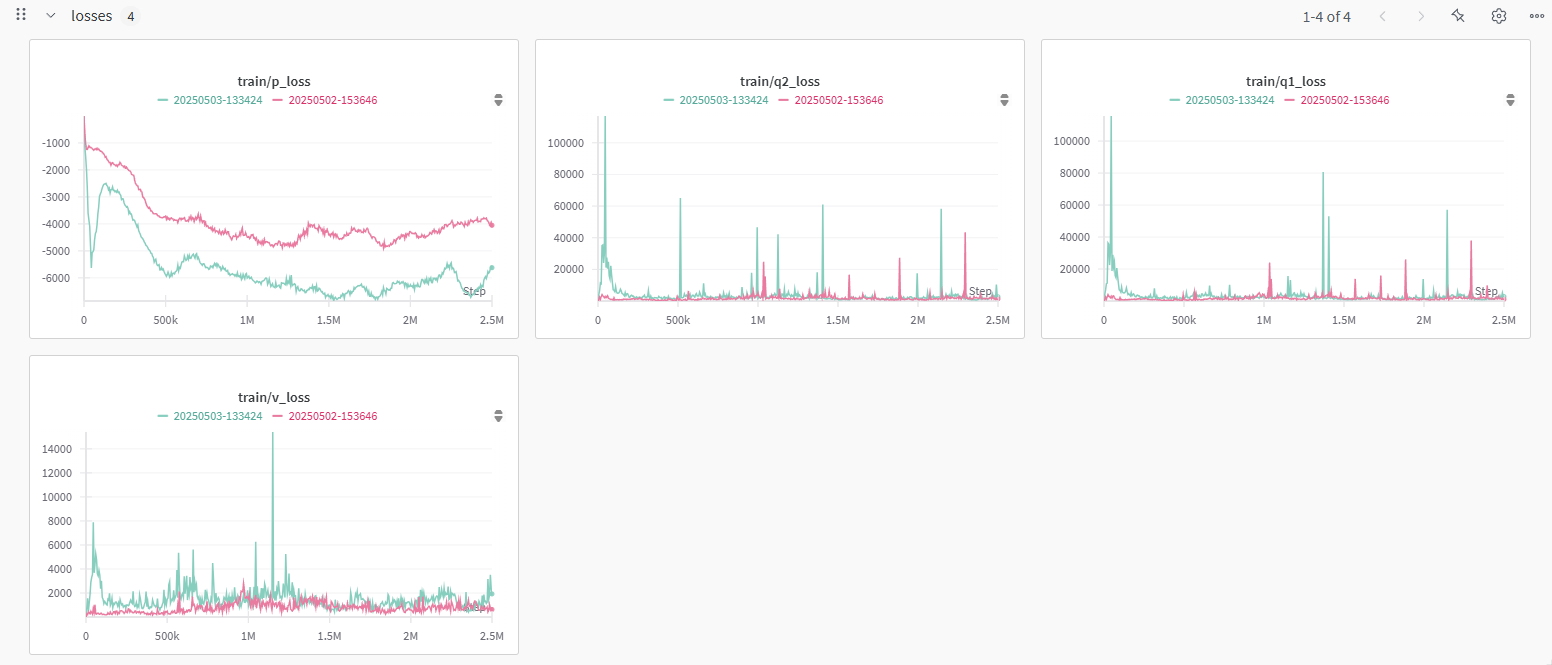
\includegraphics[width=0.85\textwidth]{AfterCoVPLossDiff.png}
    \end{figure}
\end{frame}


\begin{frame}{Change of variables}
    Adopt CoV version (Pink) has more stable gradient for P\_loss than dropped CoV version (Mint). Mint has more variance in p\_loss\_grad\_norm.
    \begin{figure}
        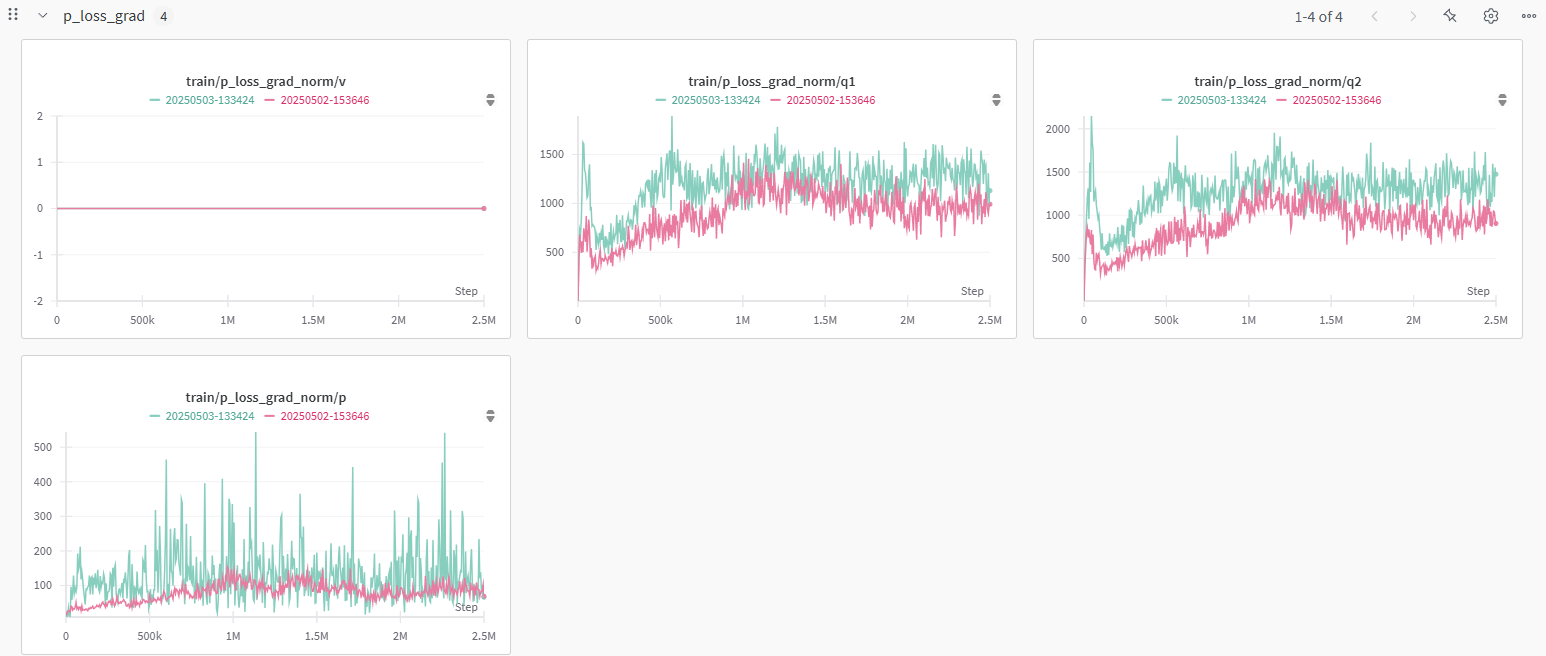
\includegraphics[width=0.75\textwidth]{MoreStablePLoss.png}
    \end{figure}

    Performance rarely slightly increases.
    \begin{figure}
        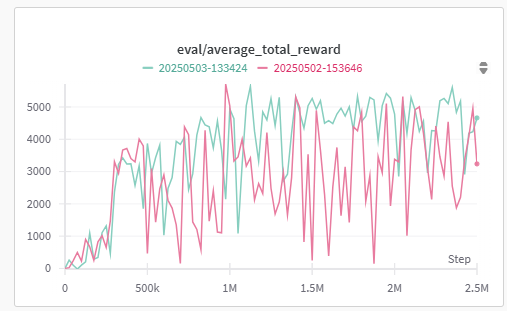
\includegraphics[width=0.45\textwidth]{CoVReturns.png}
    \end{figure}
\end{frame}

% \begin{frame}{Reproducibility}
%     In RTX-3060 GPU, in default setting, F.Linear operation doesn't guarantee reproducibility
%     \begin{columns}
%         \begin{column}{0.5\textwidth}
%             \begin{figure}
%                 \centering
%                 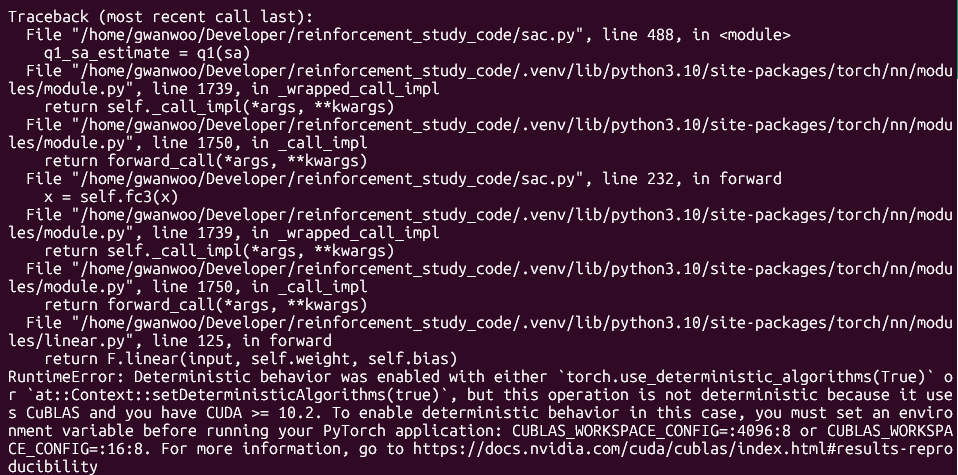
\includegraphics[width=1.0\textwidth]{CuBLASIssue.png}
%             \end{figure}
%         \end{column}
%         \begin{column}{0.5\textwidth}
%             \begin{figure}
%                 \begin{center}
%                     
\includegraphics[width=1.0\textwidth]{CublasEnvironmentVariable.png}
%                 \end{center}
%             \end{figure}
%         \end{column}
%     \end{columns}
%     \begin{itemize}
%         \item To guarantee reproducibility, need to set environment variable "CUBLAS\_WORKSPACE\_CONFIG" as ":4096:8" or "16:8"
%         \item But occurs slow down of training as nearly $2/3$
%     \end{itemize}
% \end{frame}


% \begin{frame}{Check loss function}
%     Update rule for value function $Q$ is
%     \[
%     \begin{gathered}
%         J_Q(\theta) = \mbb{E}_{(s_t, a_t) \sim \mathcal{D}}\left[\frac{1}{2} \left(  Q_\theta (s_t, a_t) - \hat{Q}  (s_t, a_t) \right)^2 \right] \\
%         \hat{\nabla}_\theta J_Q(\theta) = \nabla_\theta Q_\theta (s_t, a_t) \left( Q_\theta(s_t, a_t) -r(s_t, a_t) -\gamma V_{\hat{\psi}}(s_{t+1})  \right)
%     \end{gathered}
%     \]

% \end{frame}


\begin{frame}{Check loss function}
    Update rule for value function $V$ is
    \[
    \begin{gathered}
        J_V(\psi) = \mbb{E}_{s_t \sim \mathcal{D}} \left[ \frac{1}{2}\left(V_\psi (s_t) - \mbb{E}_{a_t \sim \pi_\phi} \left[Q_\theta (s_t, a_t) - \log{(\pi_\phi (a_t |s_t))}\right]\right)^2\right] \\
        \hat{\nabla}_\psi J_V(\psi) = \nabla_\psi V_\psi (s_t) \left(V_\psi (s_t) - Q_\theta (s_t, a_t) + \log{\pi_\phi (a_t|s_t)}\right)
    \end{gathered}
    \]

    \begin{figure}
        \centering
        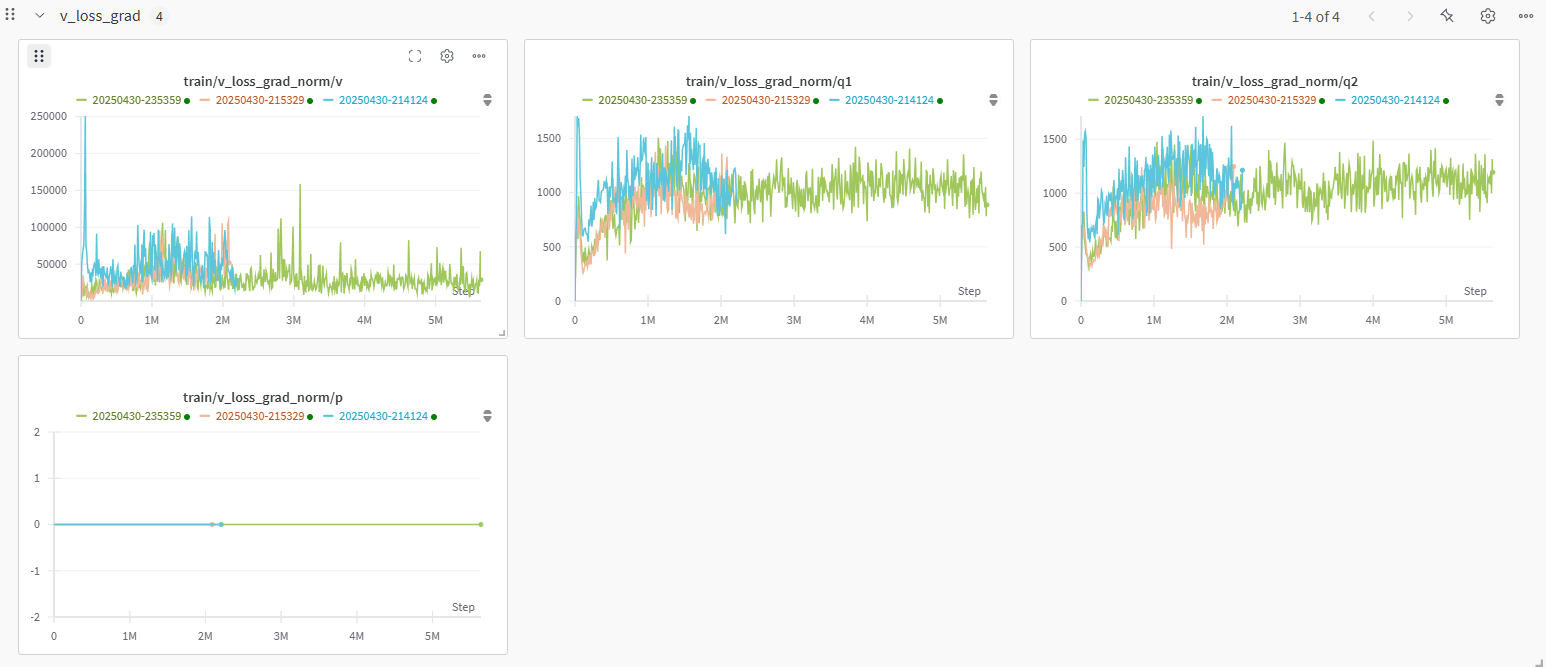
\includegraphics[width=0.9\textwidth]{fig4.png}
    \end{figure}

    \begin{itemize}
        \item There should be no gradient in policy network (p, q1, q2)
        \item But it seems there also exists gradients for Q network (q1, q2)
        \item Something is going to wrong
    \end{itemize}
\end{frame}


\begin{frame}{Check loss function}
    The code snippet for calculating V loss seems clear.

    \begin{itemize}
        \item Gradient for Q networks are not calculated because every forward operation is performed within "torch.no\_grad()" context.
        \item There only exists gradient for V network
    \end{itemize}

    \begin{figure}
        \centering
        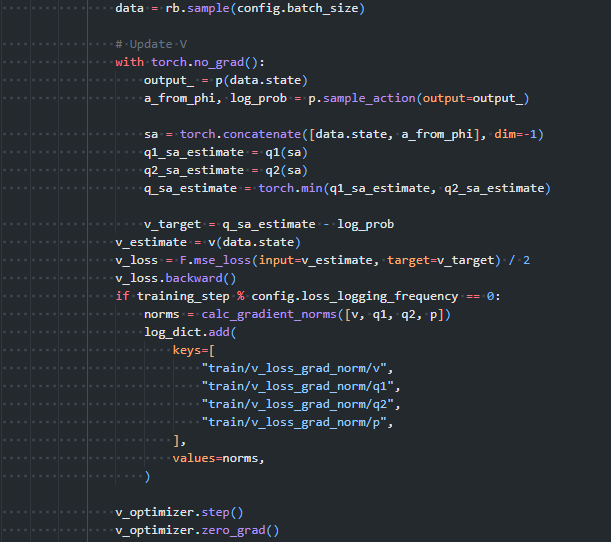
\includegraphics[width=0.65\textwidth]{fig5.png}
    \end{figure}
\end{frame}

\begin{frame}{Check loss function}
    Check the algorithm
    \begin{figure}
        \centering
        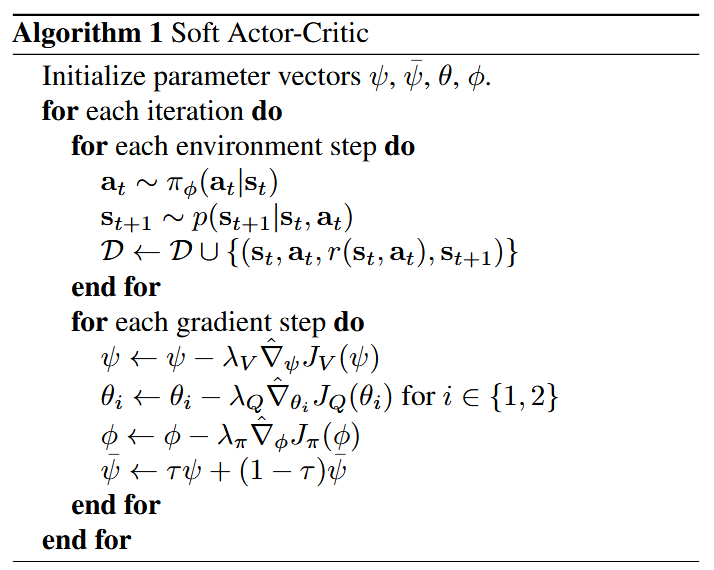
\includegraphics[width=0.6\textwidth]{fig6.png}
    \end{figure}
    Before update V($\psi$) network, Policy network($\phi$) is preceded.
    \begin{itemize}
        \item It is possible that gradient of Q network remains, which is produced by previous loss function (Policy Loss)
    \end{itemize}
\end{frame}

\begin{frame}{Check loss function}
    The objective function and its gradient with respect to policy network $(\phi)$ is
    \[
    \begin{gathered}
        J_\pi(\phi) = \mbb{E}_{s_t \sim \mathcal{D}} [\log{\pi_\phi (f_\phi (\epsilon_t;s_t)| s_t)} - Q_\theta (s_t, f_\phi (\epsilon_t; s_t))]\\
        \hat{\nabla}_\phi J_\pi (\phi) = \nabla_\phi \log{\pi_\phi (a_t|s_t)} + (\nabla_{a_t} \log{\pi_\phi (a_t|s_t)} - \nabla_{a_t} Q(s_t, a_t))\nabla_\phi f_\phi (\epsilon_t; s_t)
    \end{gathered}
    \]

    \begin{columns}[c]
        \begin{column}{0.5\textwidth}
            \begin{figure}
                \centering
                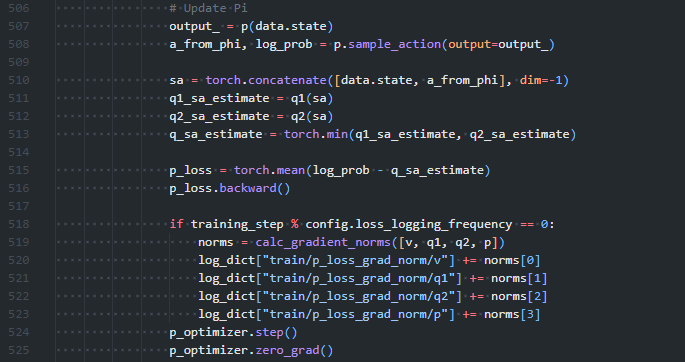
\includegraphics[width=1.0\textwidth]{fig7.png}
            \end{figure}
        \end{column}
        \begin{column}{0.5\textwidth}
            \begin{figure}
                \centering
                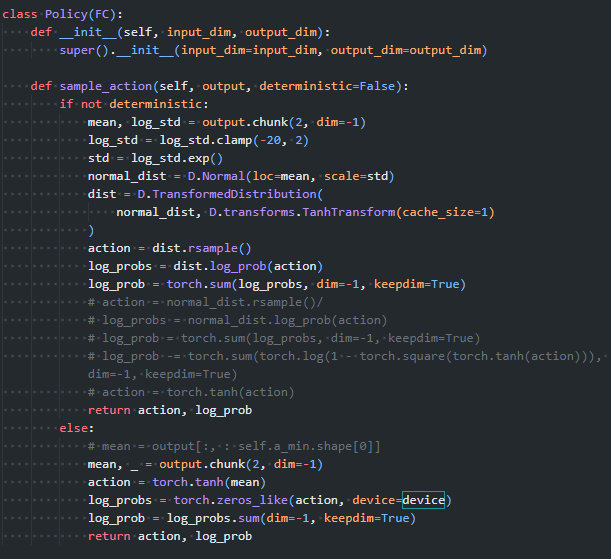
\includegraphics[width=0.9\textwidth]{fig8.png}
            \end{figure}
        \end{column}
    \end{columns}

    \begin{itemize}
        \item Gradient for $\text{"log\_prob"}$ is correspond to \(\nabla_\phi \log{\pi_\phi (a_t | s_t)} + \nabla_{a_t} \log{\pi_\phi (a_t|s_t)} \nabla_{\phi} f_\phi (\epsilon_t; s_t)  \)
        \item Gradient for  $\text{"q\_sa\_estimate"}$ is correspond to 
        \( \nabla_{a_t} Q(s_t, a_t) \nabla_\phi f_\phi (\epsilon_t; s_t) \)
    \end{itemize}
\end{frame}

\begin{frame}{Check loss function}
    \[
    \begin{gathered}
        J_\pi(\phi) = \mbb{E}_{s_t \sim \mathcal{D}} [\log{\pi_\phi (f_\phi (\epsilon_t;s_t)| s_t)} - Q_\theta (s_t, f_\phi (\epsilon_t; s_t))]\\
        \hat{\nabla}_\phi J_\pi (\phi) = \nabla_\phi \log{\pi_\phi (a_t|s_t)} + (\nabla_{a_t} \log{\pi_\phi (a_t|s_t)} - \nabla_{a_t} Q(s_t, a_t))\nabla_\phi f_\phi (\epsilon_t; s_t)
    \end{gathered}
    \]
    
    \begin{figure}
        \centering
        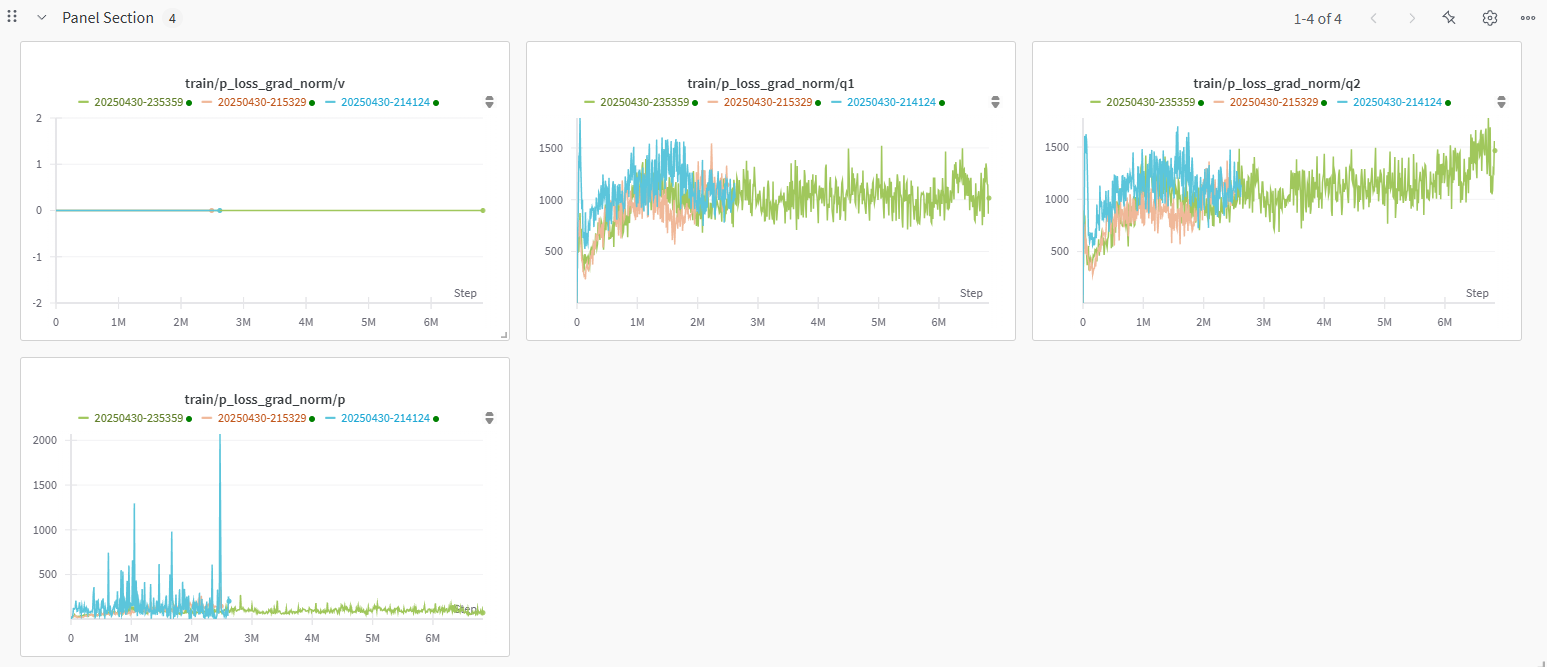
\includegraphics[width=0.9\textwidth]{fig9.png}
    \end{figure}

    \begin{itemize}
        \item There exists gradient in Q networks (q1, q2)
        \item It seems natural that gradient for q1, q2 is not zero because $\hat{\nabla_\phi} J_\pi (\phi)$ includes $\nabla_{a_t}Q(s_t, a_t)$
    \end{itemize}
\end{frame}


\begin{frame}{Check loss function}
    Then why gradient of Q network is remained?
    \begin{figure}
        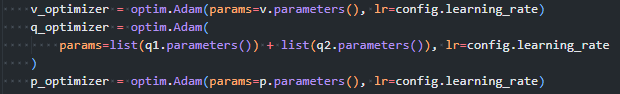
\includegraphics[width=0.6\textwidth]{POptimizerMistake1.png}
    \end{figure}
    \begin{figure}
        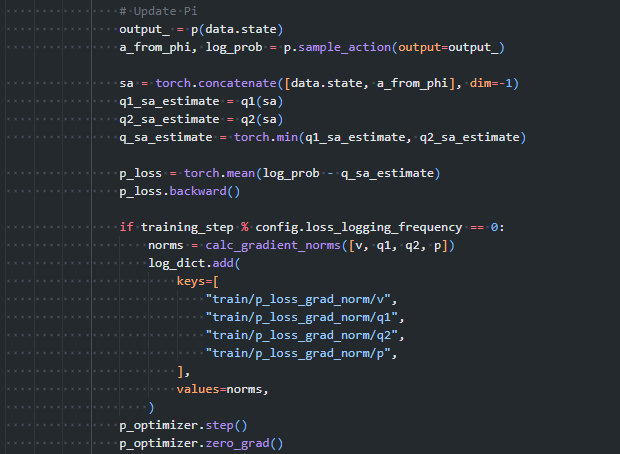
\includegraphics[width=0.6\textwidth]{POptimizerMistake2.png}
    \end{figure}

    It is because \ti{optimizer.zero\_grad()} function only clear gradient of its parameters.
    \begin{itemize}
        \item In this experinent, \ti{p\_optimizer.zero\_grad()} function only clear the gradient of Policy Network
        \item So, gradient of Q network still remains
    \end{itemize}
\end{frame}

\begin{frame}{Check loss function}
    \begin{columns}
        \begin{column}[]{0.4\textwidth}
            \begin{itemize}
                \item Remained gradient of Q network is measured (red line). 
                \item And this remained gradient is accumulated with another gradient calculated from Q loss (blue line)
                \item This mixed gradient from two different loss function distort the desired true gradient of Q network (yellow line)
            \end{itemize}
            Note that, gradient is not overwritten remained. it is accumulated with previous one.
        \end{column}
        \begin{column}{0.6\textwidth}
            \begin{figure}
                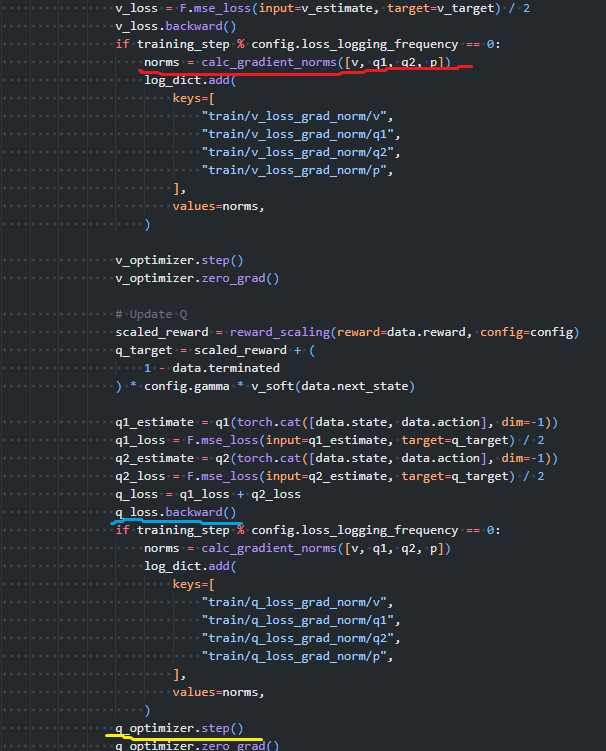
\includegraphics[width=1.0\textwidth]{VlossQloss.png}
            \end{figure}
        \end{column}
    \end{columns}
\end{frame}

\begin{frame}{Check loss function}
    The desired true gradient of Q network is 
    \[
     \hat{\nabla}_{\theta_i} J_Q (\theta_i) = \nabla_{\theta_i} Q_{\theta_i} (s_t, a_t) \left(Q_{\theta_i}(s_t, a_t) - r(s_t, a_t) - \gamma V_{\hat{\psi}}(s_{t+1}) \right)
    \]
    And previous wrong gradient of Q network is calculated by
    \[
        \nabla_{\theta_i} Q_{\theta_i} (s_t, a_t) \left(Q_{\theta_i}(s_t, a_t) - r(s_t, a_t) - \gamma V_{\hat{\psi}}(s_{t+1}) \right) - \nabla_{a_t} Q(s_t, a_t) \nabla_\phi f_\phi (\epsilon_t; s_t)
    \]
    where unwanted gradient term $- \nabla_{a_t} Q(s_t, a_t) \nabla_\phi f_\phi (\epsilon_t; s_t)$ is appended
\end{frame}

\begin{frame}{Check loss function}
    Fix this unwanted ramaining of gradient
    \begin{figure}
        
\includegraphics[width=0.8\textwidth]{AllOptimizerUpdate1.png}
    \end{figure}
    \begin{figure}
        
\includegraphics[width=0.8\textwidth]{AllOptimizerUpdate2.png}
    \end{figure}
    \begin{figure}
        
\includegraphics[width=0.8\textwidth]{AllOptimizerUpdate3.png}
    \end{figure}

    After each network update, clear all network's gradient via call \ti{zero\_grad()} method of all optimizers
\end{frame}

\begin{frame}{Check loss function}
    \begin{columns}
        \begin{column}{0.5\textwidth}
            \begin{itemize}
                \item It seems there is no dramatic increasing
                \item Comparing the scale of q loss gradient norms from each q\_loss and p\_loss, Norm of gradient from q\_loss is significantly bigger than one from p\_loss
                \item Leading no improvement
            \end{itemize}
        \end{column}
        \begin{column}{0.5\textwidth}
            \begin{figure}
                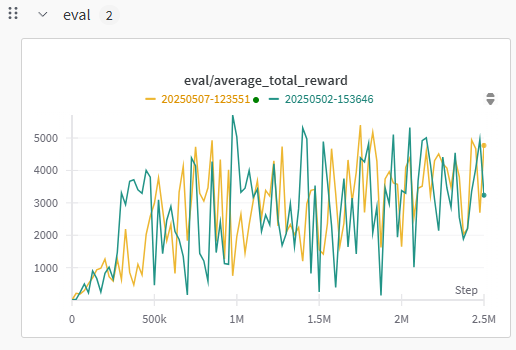
\includegraphics[width=0.75\textwidth]{NoBigDiffafterLossFix.png}
            \end{figure}
        \end{column}
    \end{columns}
    \begin{figure}
        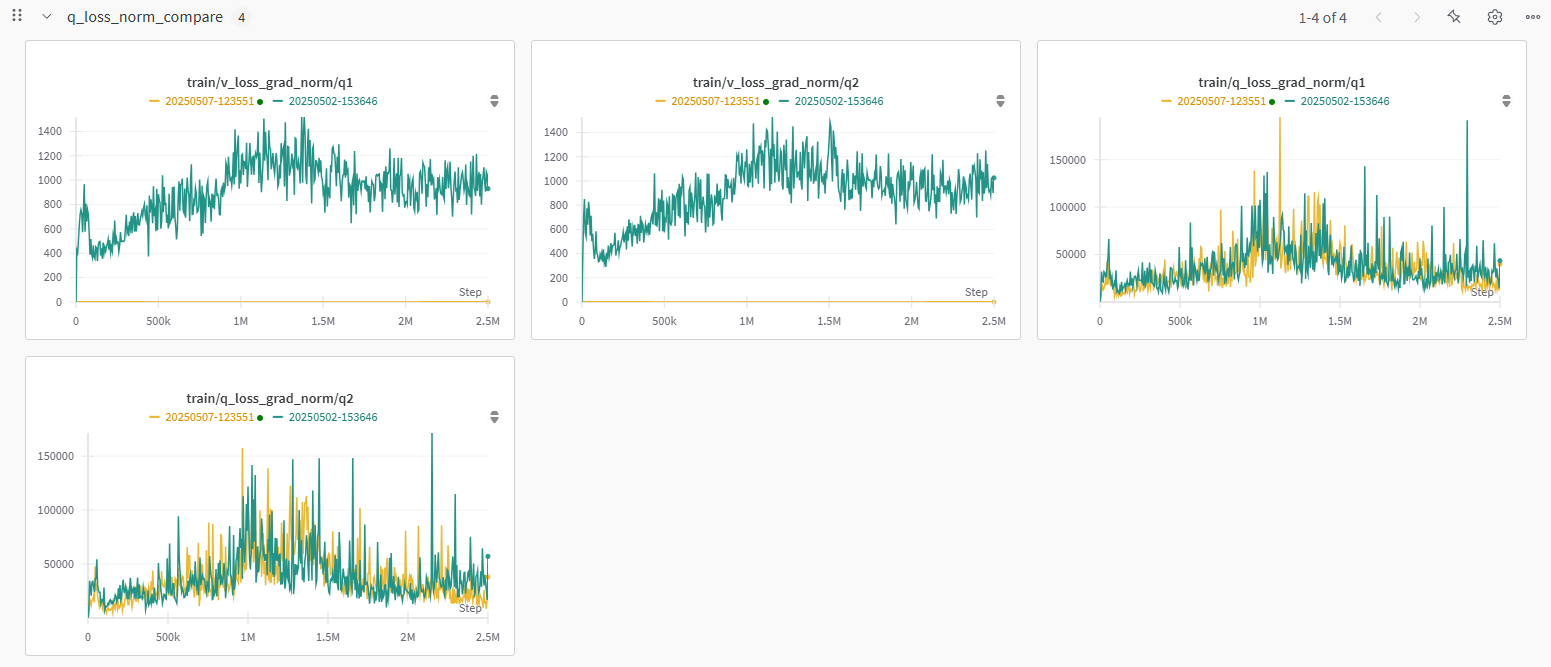
\includegraphics[width=0.86\textwidth]{CompareQGradNorm.png}
    \end{figure}
\end{frame}

\begin{frame}{More stuff to experiment}
    \begin{itemize}
        \item Implement discrete version of SAC
        \item Experiment in more harder environments (It seems walker2d is too easy task to SAC algorithm)
        \item Reward Scaling
    \end{itemize}
\end{frame}


% \begin{frame}{Robust for variant seeds}
%     \begin{itemize}
%         \item When run with same seed, same performance is obtained
%         \item It seems seed fix is well done
%     \end{itemize}
%     \begin{figure}
%         \centering
%         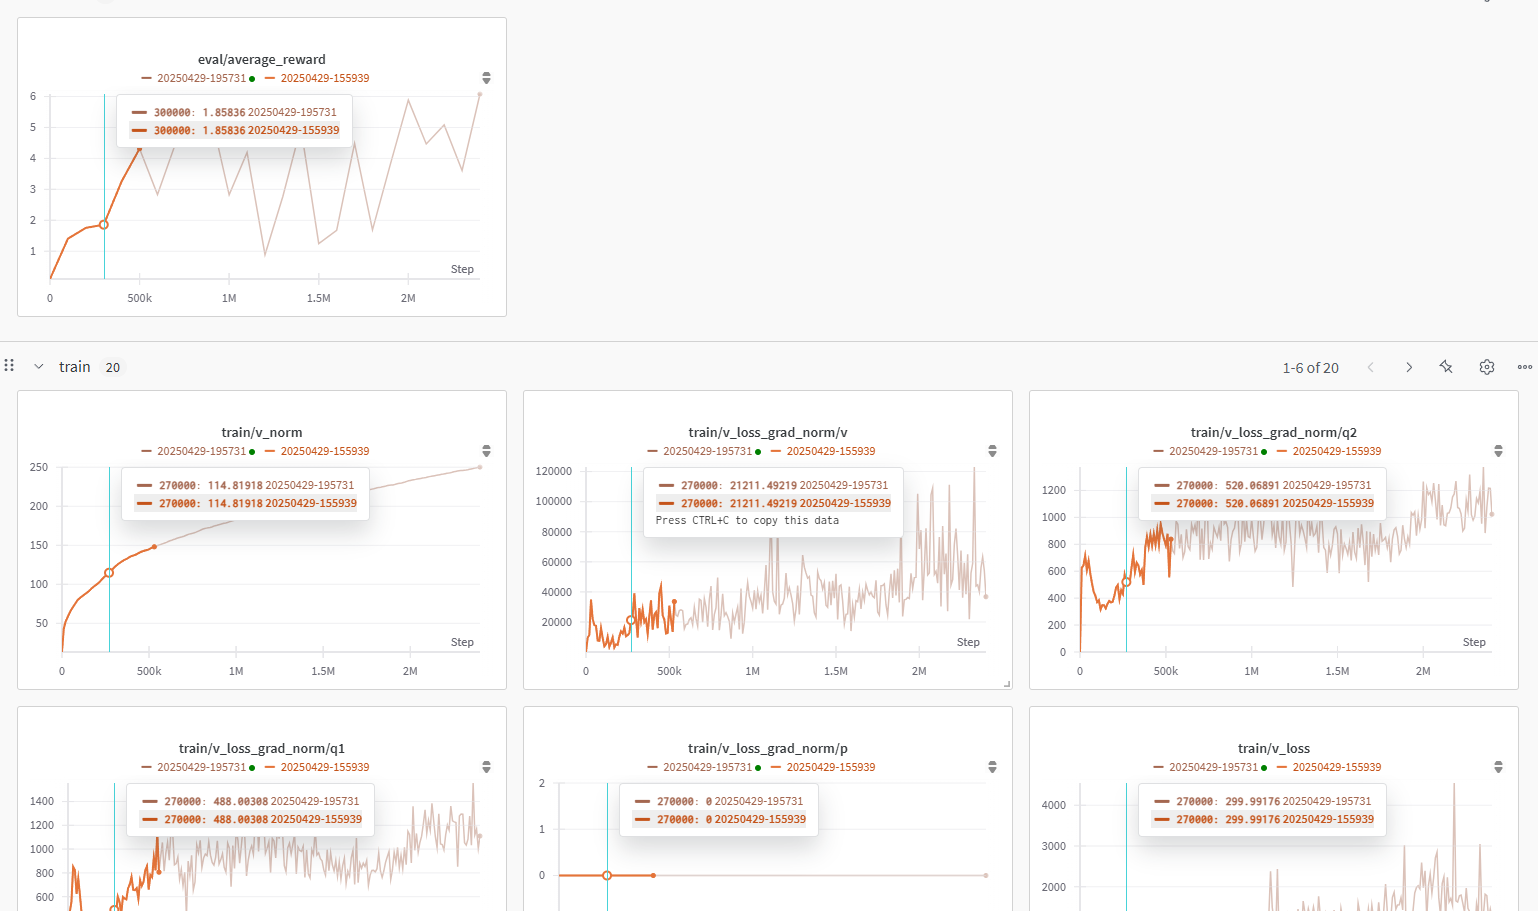
\includegraphics[width=0.8\textwidth]{fig1.png}
%     \end{figure}

%     Average reward is calculated by
%     $\frac{\sum_{i=1}^T r_i}{T}$, where $T$ is terminated time step.
% \end{frame}

% \begin{frame}{Robust for variant seeds}
%     \begin{itemize}
%         \item With variant seeds, different performance is obtained
%         \item But shows \tb{similar performance}
%         \item One of the important property of SAC is robust performance and this experiment shows that point
%     \end{itemize}

%     \begin{figure}
%         \centering
%         
\includegraphics[width=0.8\textwidth]{fig2.png}
%     \end{figure}
% \end{frame}

\end{document}